\documentclass[fleqn,addpoints]{exam}

\usepackage{graphicx}
\usepackage{float}
\usepackage{amsmath}
\usepackage{cancel}
\usepackage{polynom}
\usepackage{caption}

\printanswers

\ifprintanswers 
\usepackage{2in1, lscape} 
\fi

\title{Math 115 Homework 11}
\date{December 28, 2010}

\begin{document}

\maketitle
 

\ifprintanswers
\else
\section{Reading}
Read Larson/Hostetler Section 2.3.

\section{Homework}

\begin{itemize}
  \item Larson/Hostetler, pp 233-235: 10-11, 18, 21-25, 39-42, 48, 51-55, 61-62, 71-72
  \item Faires/DeFranza, p 121: 13-15
\end{itemize}

\section{Calculator Problems (optional)}
\begin{itemize}
  \item Larson/Hostetler, pp 233-235: 67-70
\end{itemize}

\fi

\ifprintanswers

\section{Larson/Hostetler}

\begin{description}
\item[10]
\[ 
  \polylongdiv{6x^3 - 16x^2 + 17x - 6}{3x-2} 
\]

\item[11]
\[ 
  \polylongdiv{x^4 + 5x^3 + 6x^2 - x - 2}{x+2} 
\]

\item[18]
\[ 
  \polylongdiv{x^5+7}{x^3-1} 
\]

\item[21]
\[
  \polyhornerscheme[x=5]{3x^3-17x^2+15x-25} \\
\]
\[
  3x^2 - 2x + 5
\]

\item[22]
\[
  \polyhornerscheme[x=-3]{5x^3+18x^2+7x-6} \\
\]
\[
  5x^2 + 3x - 2
\]

\item[23]
\[
  \polyhornerscheme[x=-2]{4x^3+8x^2-9x-18} \\
\]
\[
  4x^2-9
\]

\item[24]
\[
  \polyhornerscheme[x=2]{9x^3-18x^2-16x+32} \\
\]
\[
  9x^2-16
\]

\item[25]
\[
  \polyhornerscheme[x=-10]{-x^3+75x-250} \\
\]
\[
  -x^2+10x-25
\]

\item[39]
\[
  \polyhornerscheme[x=4]{x^3-x^2-14x+11} \\
\]
\[
  f(x) = (x^2+3x-2)(x-4) + 3
\]

\item[40]
\[
  \polyhornerscheme[x=-2]{x^3-5x^2-11x+8} \\
\]
\[
  f(x) = (x^2-7x+3)(x+2) + 2
\]

\item[41]
\[
  \polyhornerscheme[x=-\frac{2}{3}]{15x^4+10x^3-6x^2+14} \\
\]
\[
  f(x) = (15x^3 - 6x+4) \left( x+\frac{2}{3} \right) + \frac{34}{3}
\]

\item[42]
\[
  \polyhornerscheme[x=\frac{1}{5}]{10x^3-22x^2-3x+4} \\
\]
\[
  f(x) = (10x^2-20x-7) \left( x-\frac{1}{5} \right) + \frac{13}{5}
\]

\item[48]
For the ``verify using another method'' part, it's easiest to do a little factoring of the equation first.  Then you
don't need to do as much aritimetic on big numbers:

\begin{align*}
  f(x) &= x^6-4x^4+3x^2 + 2 \\
       &= x^2(x^4-4x^2+3) + 2 \\
       &= x^2(x^2-3)(x^2-1) + 2 \\
\end{align*}

\begin{description}
\item[a]
\[
  \polyhornerscheme[x=2]{x^6-4x^4+3x^2+2} \\
\]

So $f(2) = 14$.  

Verify:
\[
  f(2) = 2^2(2^2-3)(2^2-1) + 2 = 4(1)(3) + 2 = 14 \\
\]

\item[b]
\[
  \polyhornerscheme[x=-4]{x^6-4x^4+3x^2+2} \\
\]

So $f(-4) = 3122$.  

Verify:
\[
  f(2) = (-4)^2((-4)^2-3)((-4)^2-1) + 2 = 16(13)(15) + 2 = 3122 \\
\]

\item[c]
\[
  \polyhornerscheme[x=3]{x^6-4x^4+3x^2+2} \\
\]

So $f(3) = 434$.  

Verify:
\[
  f(2) = (3)^2(3^2-3)(3^2-1) + 2 = 9(6)(8) + 2 = 434 \\
\]
 
\item[d]
\[
  \polyhornerscheme[x=-1]{x^6-4x^4+3x^2+2} \\
\]

So $f(-1) = 2$.  

Verify:
\[
  f(-1) = (-1)^2((-1)^2-3)((-1)^2-1) + 2 = (-2)(0) + 2 = 2 \\
\]

\end{description}

\item[51]
\[
  \polyhornerscheme[x=2]{x^3-7x+6} \\
\]

\begin{align*}
  f(x) &= (x^2 +2x -3)(x-2) \\
   &= (x+3)(x-1)(x-2) \\
\end{align*}

\item[52]
\[
  \polyhornerscheme[x=-4]{x^3-28x-48} \\
\]

\begin{align*}
  f(x) &= (x^2 - 4x - 12)(x+4) \\
       &= (x-6)(x+2)(x+4) \\
\end{align*}

\item[53]
\[
  \polyhornerscheme[x=\frac{1}{2}]{2x^3-15x^2+27x-10} \\
\]

\begin{align*}
  f(x) &= (2x^2-14x+20) \left( x-\frac{1}{2} \right) \\
       &= 2(x^2-7x+10)  \left( x-\frac{1}{2} \right) \\
       &= (x^2-7x+10)(2x-1) \\
       &= (x-5)(x-2)(2x-1) \\
\end{align*}

\item[54]
\[
  \polyhornerscheme[x=\frac{2}{3}]{48x^3-80x^2+41x-6} \\
\]

\begin{align*}
  f(x) &= (48x^2-48x+9) \left(x-\frac{2}{3} \right) \\
       &= 3(16x^2-16x+3)\left (x-\frac{2}{3} \right) \\
       &= (16x^2-16x+3)(3x-2) \\
       &= (4x-3)(4x-1)(3x-2) \\
\end{align*}

\item[55]

\begin{tabular}{c|cccc}
             & 1 & 2              & $-3$            & $-6$ \\
  $\sqrt{3}$ &   & $\sqrt{3}$     & $2\sqrt{3} + 3$ & 6 \\
  \hline
             & 1 & $2 + \sqrt{3}$ & $2\sqrt{3}$     & 0 \\
\end{tabular}

\begin{align*}
  f(x) &= (x^2 + (2+\sqrt{3})x + 2\sqrt{3})(x-\sqrt{3}) \\
       &= (x + 2)(x + \sqrt{3})(x-\sqrt{3}) \\
\end{align*}

\item[61]
\[
  \polyhornerscheme[x=5]{x^4-4x^3-15x^2+58x-40} \\
\]

\[
  f(x) = (x^3+x^2-10x+8)(x-5)
\]

\[
  \polyhornerscheme[x=-4]{x^3+x^2-10x+8} \\
\]

\begin{align*}
  f(x) &= (x^2-3x+2)(x-5)(x+4) \\
       &= (x-2)(x-1)(x-5)(x+4) \\
\end{align*}

The zeros are: $x = \{-4, 1, 2, 5 \}$

\begin{figure}[H]
  \centering
  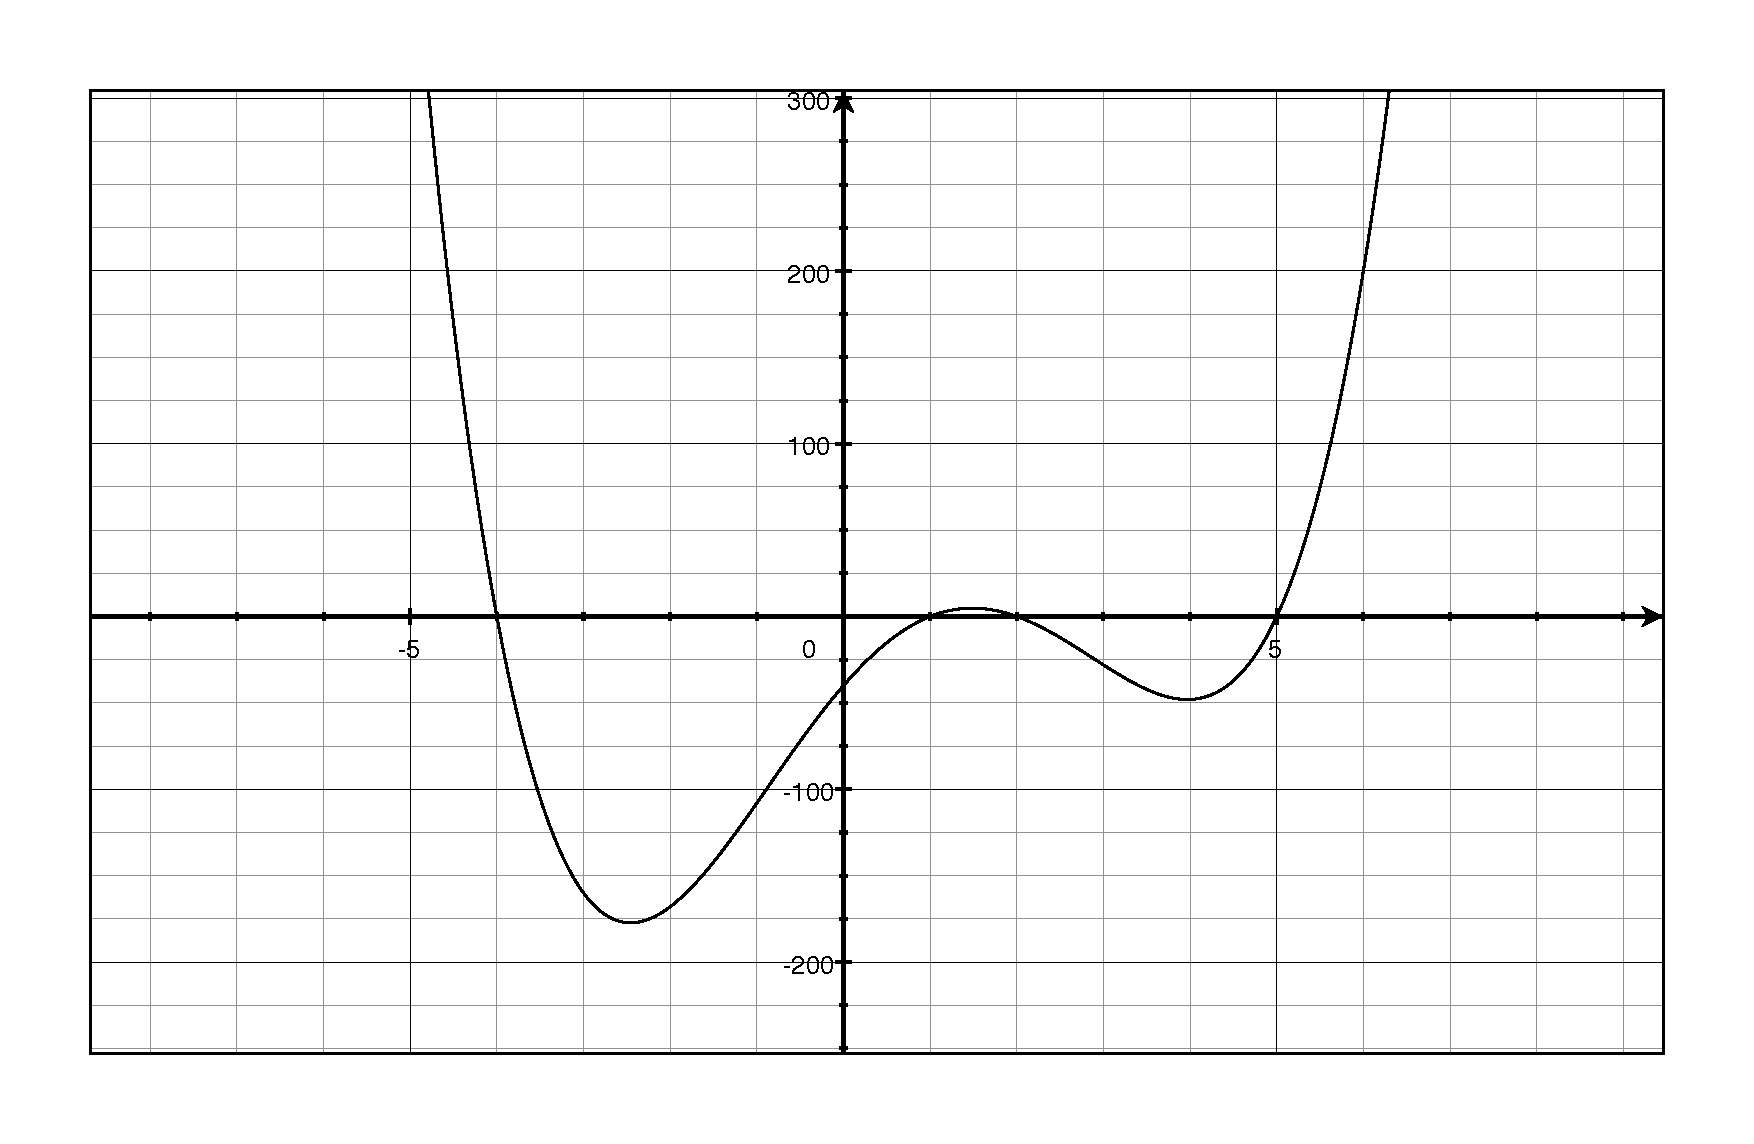
\includegraphics[width=7cm,height=5cm]{question_61.eps}
  \caption*{Question 61}
\end{figure}

\item[62]
\[
  \polyhornerscheme[x=4]{8x^4-14x^3-71x^2-10x+24} \\
\]

\[
  f(x) = (8x^3+18x^2+x-6)(x-4)
\]

\[
  \polyhornerscheme[x=-2]{8x^3+18x^2+x-6} \\
\]

\begin{align*}
  f(x) &= (8x^2+2x-3)(x-4)(x+2) \\
       &= (4x+3)(2x-1)(x-4)(x+2) \\
\end{align*}

The zeros are: $x = \left \{-2, -\dfrac{3}{4}, \dfrac{1}{2}, 4 \right \}$

\begin{figure}[H]
  \centering
  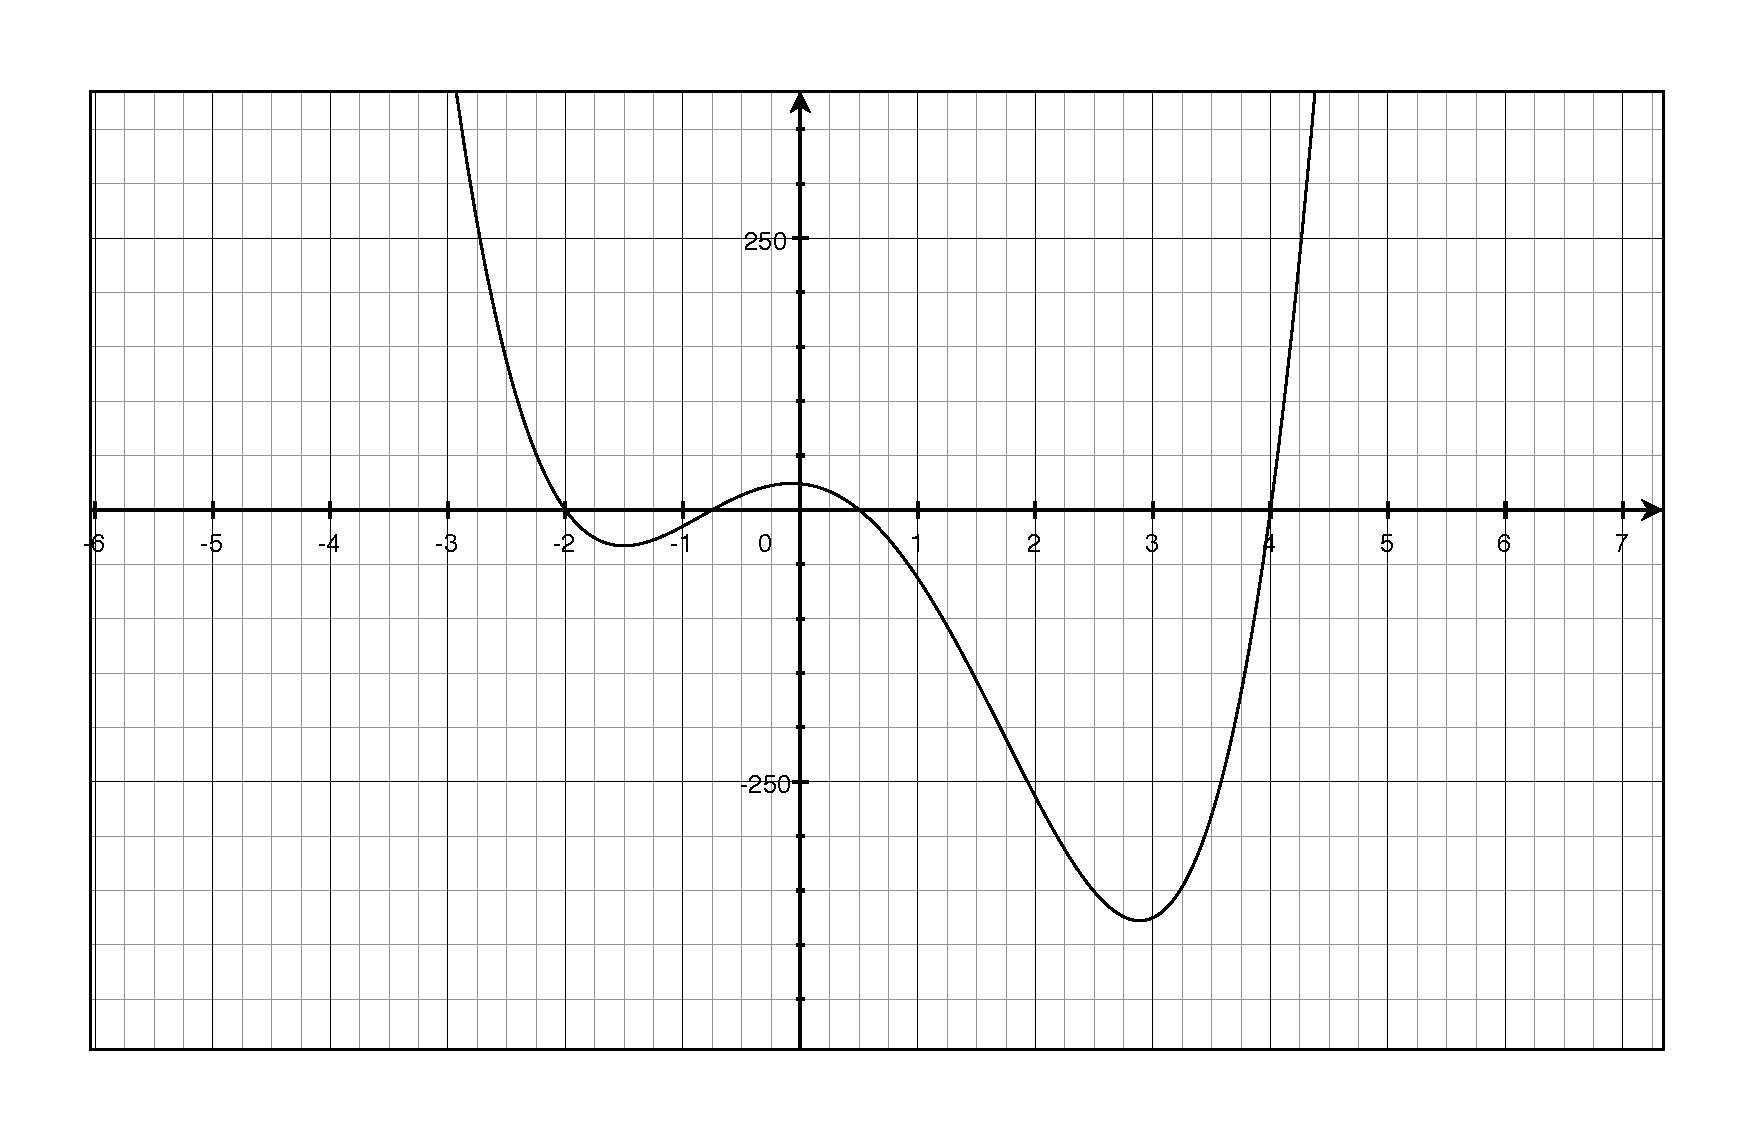
\includegraphics[width=7cm,height=5cm]{question_62.eps}
  \caption*{Question 62}
\end{figure}

\item[71]
\[ 
  \polylongdiv{4x^3 - 8x^2 + x + 3}{2x-3} 
\]

\[
  \frac{4x^3 - 8x^2 + x + 3}{2x-3} = 2x^2-x-1
\]

\item[72]
\[ 
  \polyhornerscheme[x=-8]{x^3 + x^2 - 64x - 64} \\
\]

\[
  \frac{x^3 + x^2 - 64x - 64}{x+8} = x^2-7x-8
\]

\section{Calculator Problems}
\item[67]
\begin{figure}[H]
  \centering
  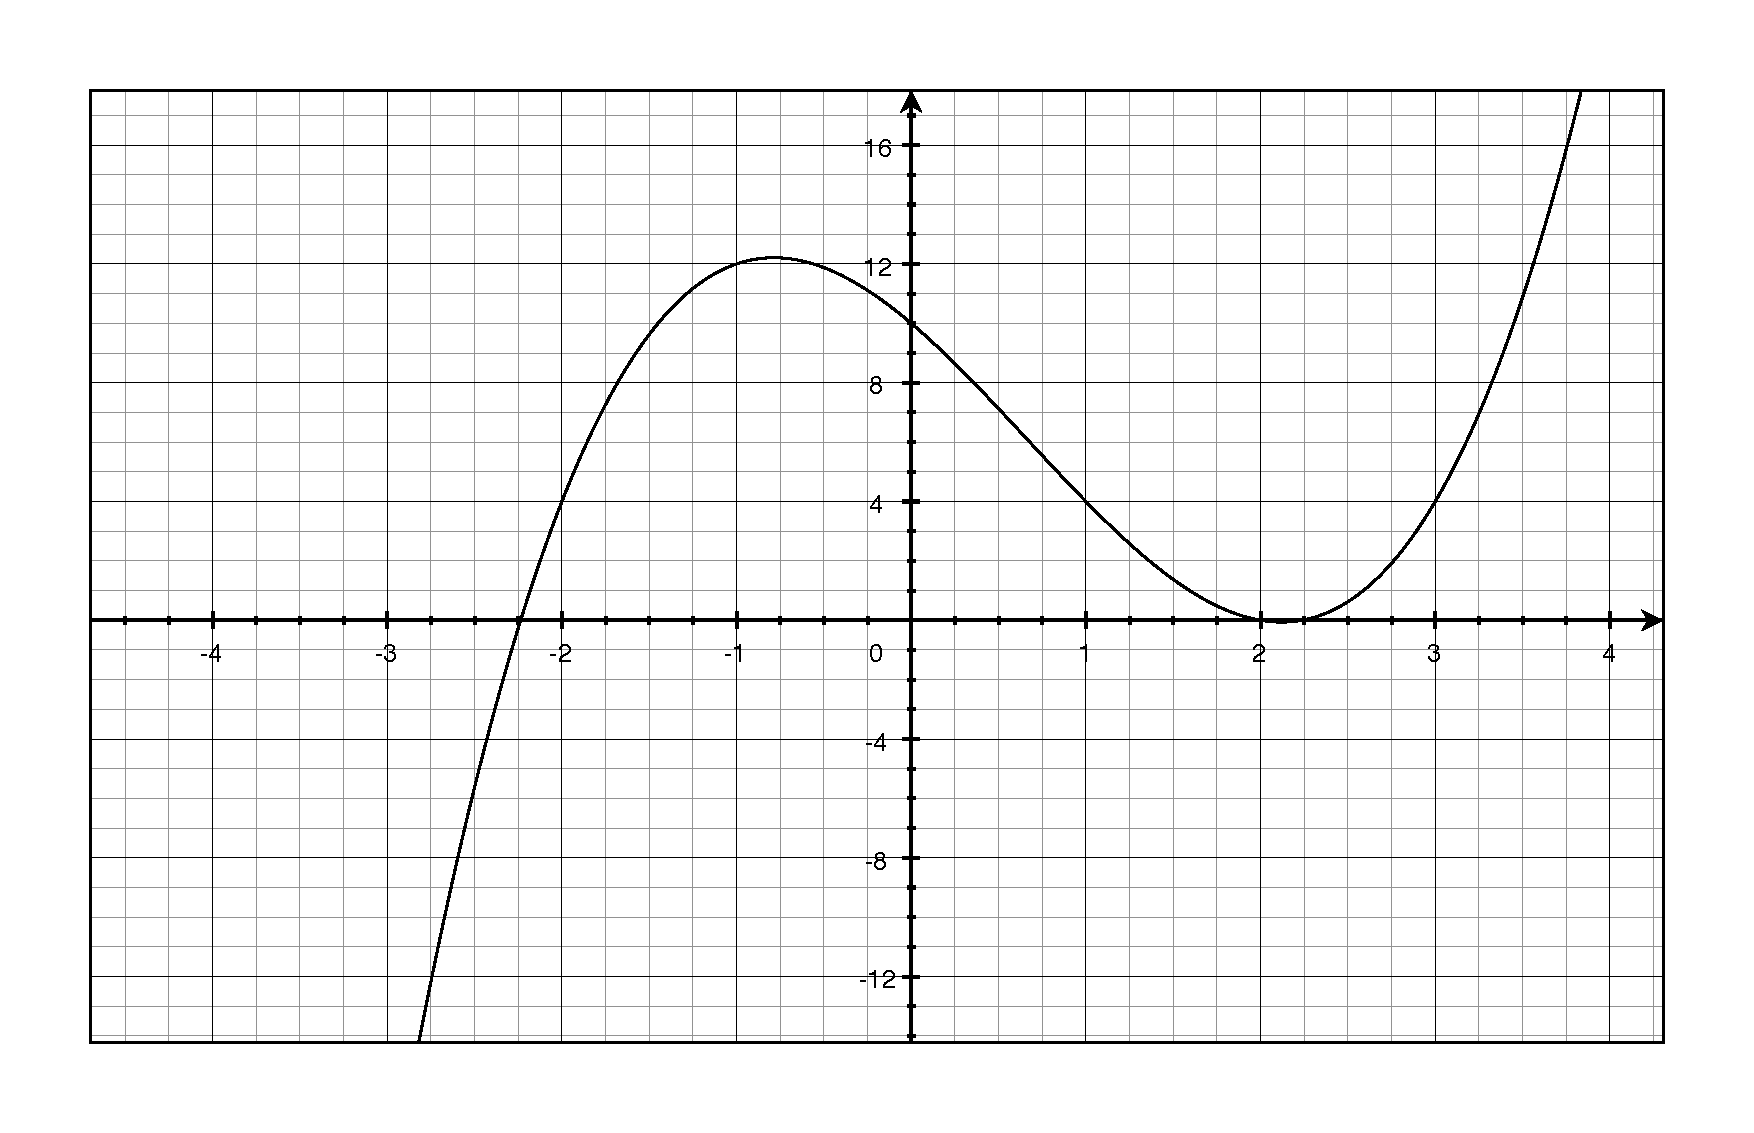
\includegraphics[width=7cm,height=5cm]{question_67.eps}
  \caption*{Question 67}
\end{figure}

From the graph, the polynomial has a root at $x=2$.

\[
  \polyhornerscheme[x=2]{x^3-2x^2-5x+10} \\
\]

\begin{align*}
  f(x) &= (x-2)(x^2-5) \\
  &= (x-2)(x + \sqrt{5})(x - \sqrt{5})
\end{align*}

\item[68]
\begin{figure}[H]
  \centering
  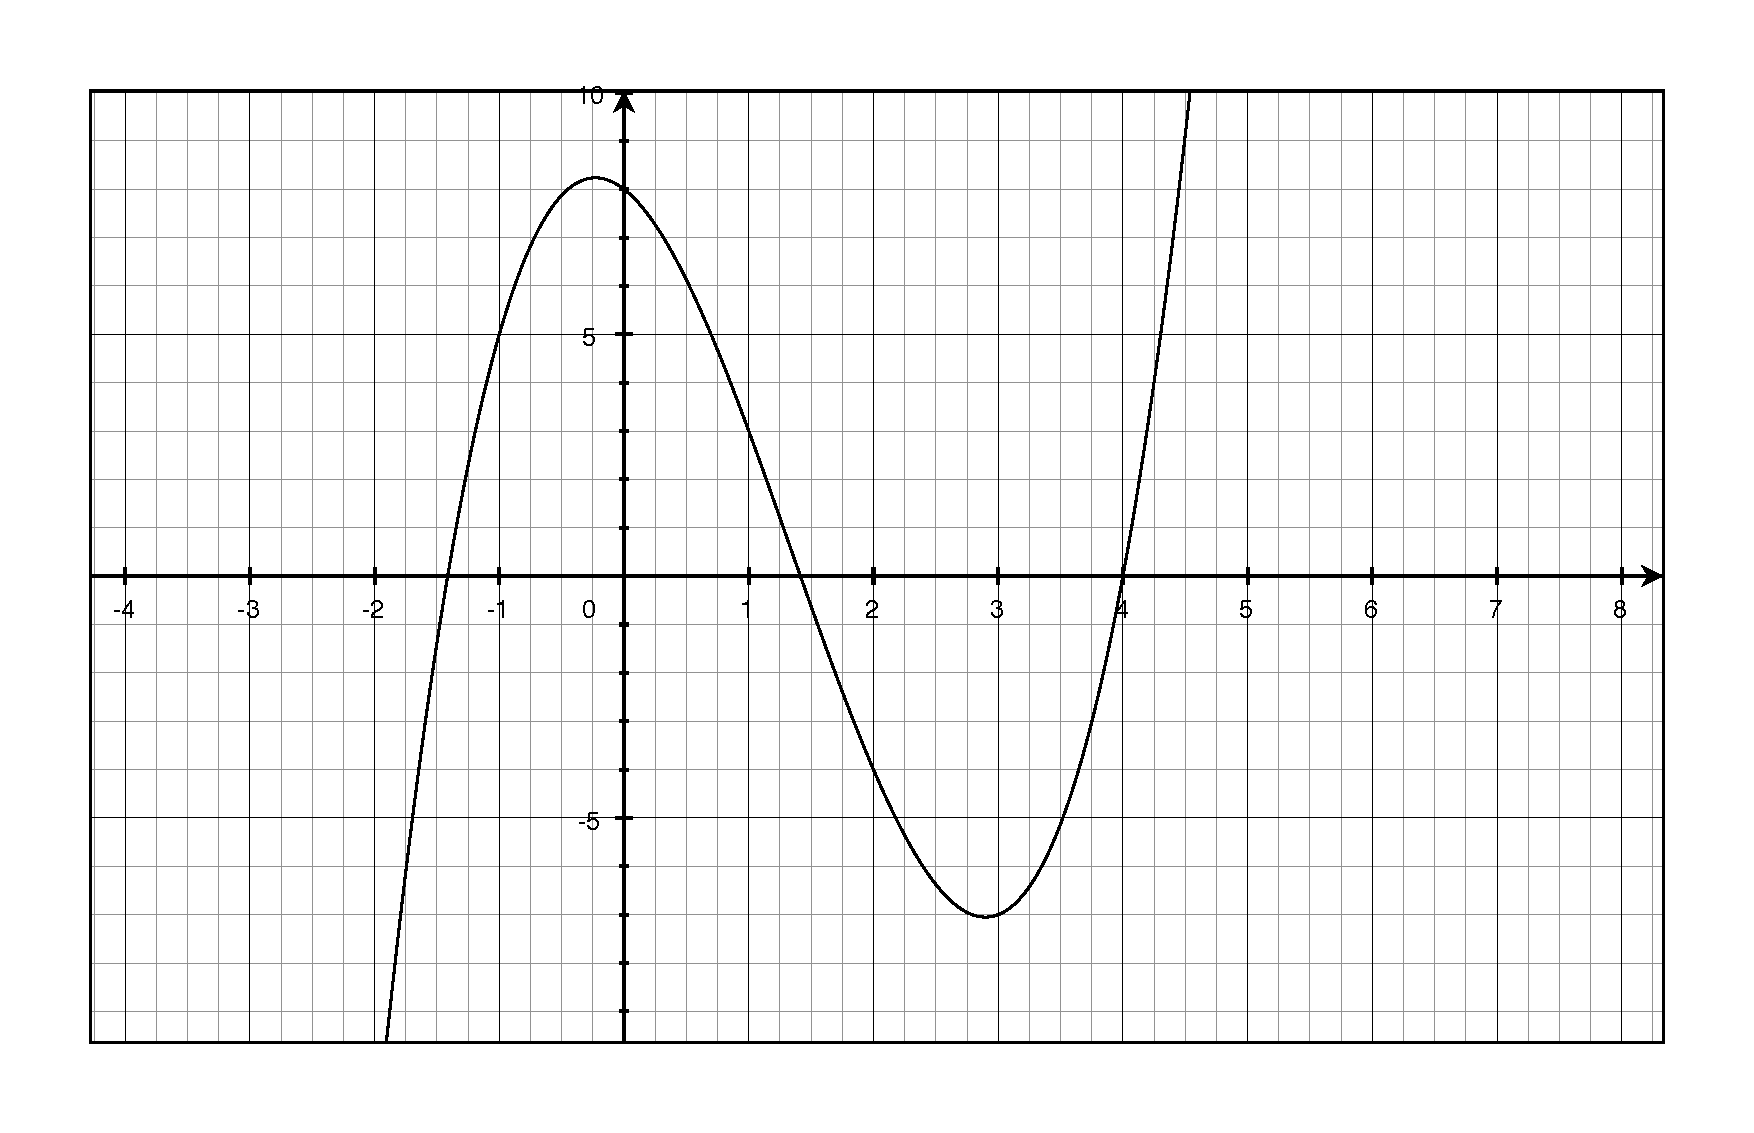
\includegraphics[width=7cm,height=5cm]{question_68.eps}
  \caption*{Question 68}
\end{figure}

From the graph, the polynomial has a root at $x=4$.

\[
  \polyhornerscheme[x=4]{x^3-4x^2-2x+8} \\
\]

\begin{align*}
  f(x) &= (x-4)(x^2-2) \\
  &= (x-4)(x + \sqrt{2})(x - \sqrt{2})
\end{align*}

\item[69]
\begin{figure}[H]
  \centering
  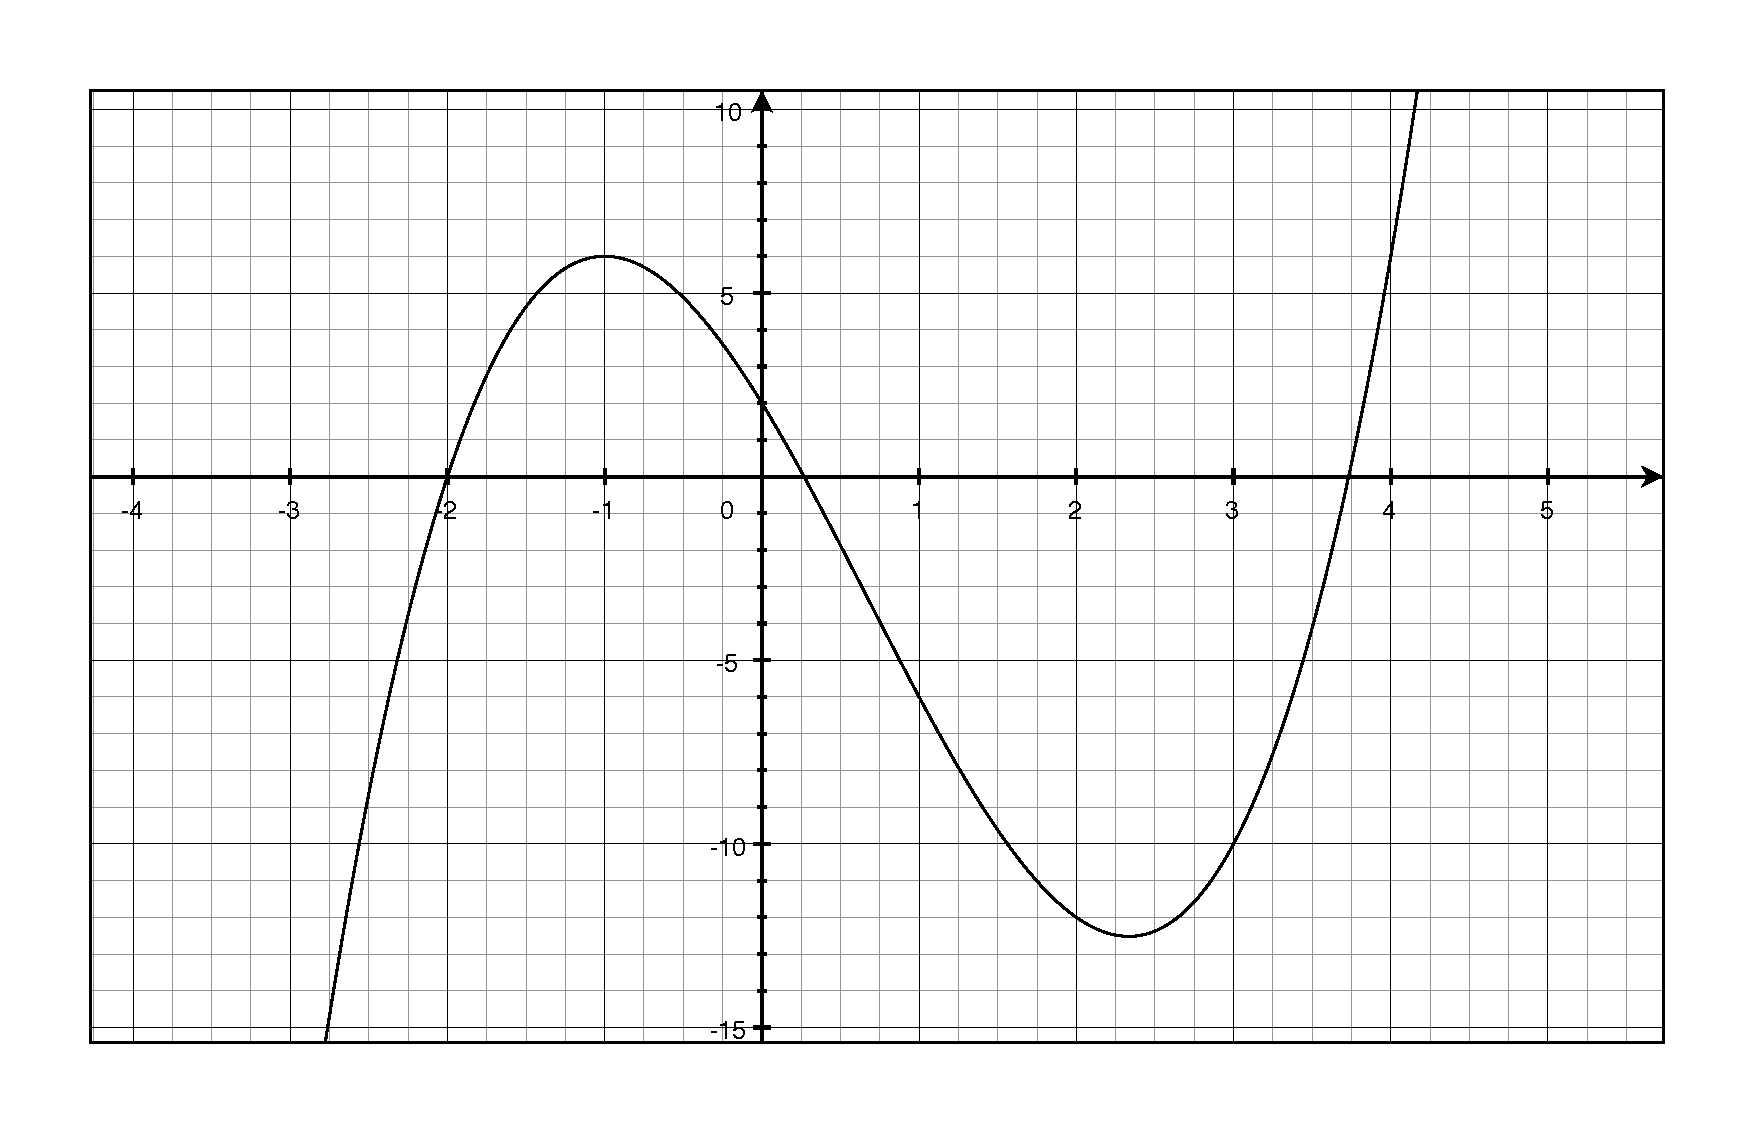
\includegraphics[width=7cm,height=5cm]{question_69.eps}
  \caption*{Question 69}
\end{figure}

From the graph, the polynomial has a root at $x=-2$.

\[
  \polyhornerscheme[x=-2]{x^3-2x^2-7x+2} \\
\]

You have to use the quadratic formula to get the remaining factors:
\begin{align*}
  h(t) &= (t+2)(t^2 - 4t + 1) \\
   &= (t+2)(t - 2 + \sqrt{3})(t - 2 - \sqrt{3}) \\
\end{align*}

\item[70]

\begin{figure}[H]
  \centering
  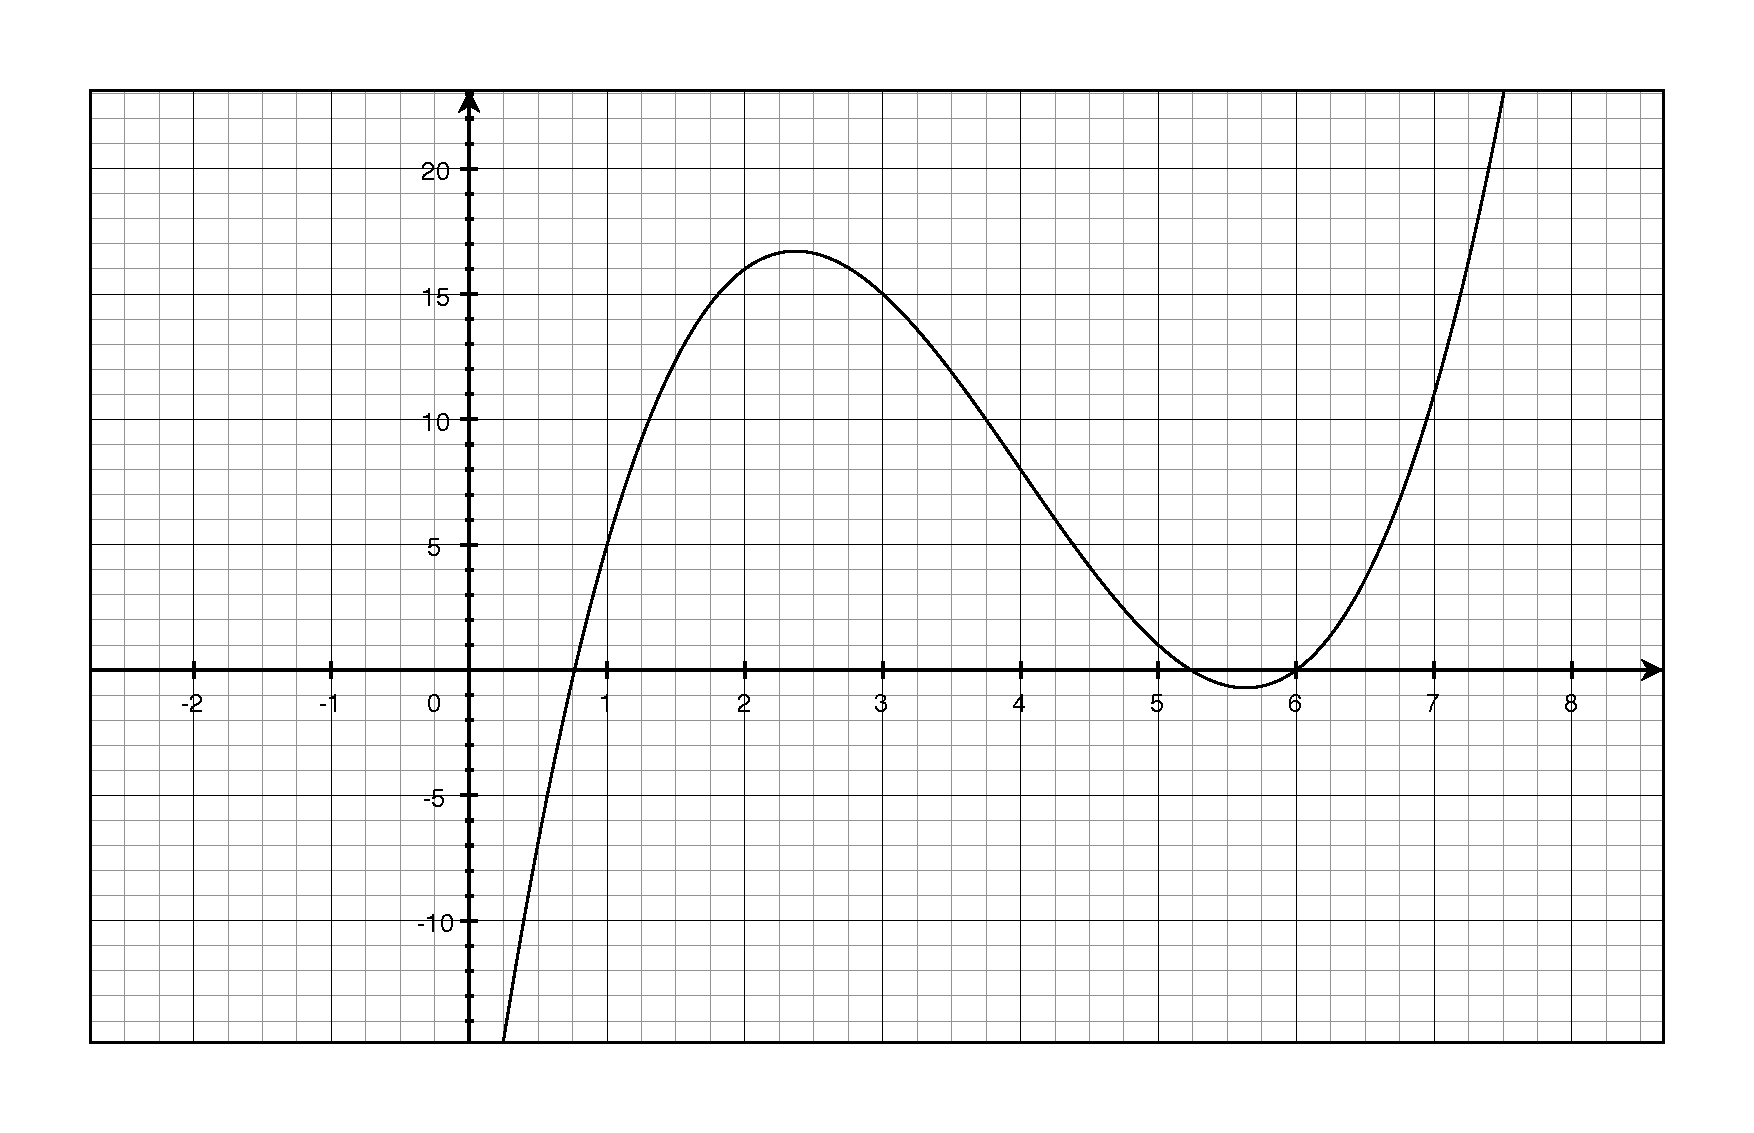
\includegraphics[width=7cm,height=5cm]{question_70.eps}
  \caption*{Question 70}
\end{figure}

From the graph, the polynomial has a root at $x=6$.

\[
  \polyhornerscheme[x=6]{x^3-12x^2+40x-24} \\
\]

You have to use the quadratic formula to get the remaining factors:
\begin{align*}
  f(s) &= (s-6)(s^2 - s + 4) \\
   &= (s+2)(s - 3 + \sqrt{5})(s - 3 - \sqrt{5}) \\
\end{align*}

\pagebreak

\section{Faires/DeFranza}

\item[13]

There are many polynomails that would work.  The simplest one is this:
\[
  P(x) = (x-1)(x+1)(x-2)
\]

The polynomial could be multiplied by a constant and still have the same zeros.  So $Q(x) = 2(x-1)(x+1)(x-2)$, for
example, would also work.  You could also add additional factors if you felt like it.  $R(x) = (x-1)(x+1)(x-2)(x+17)(x-5)$, for example
would also work. 

But, sticking with the simplest solution, here are a few points:
\begin{tabular}{|c|c|c|c|c|}
\hline
  x & -2  & 0 & $3/2$  & 3 \\
\hline
  y & -12 & 2 & $-5/8$ & 8 \\
\hline
\end{tabular}

\begin{figure}[H]
  \centering
  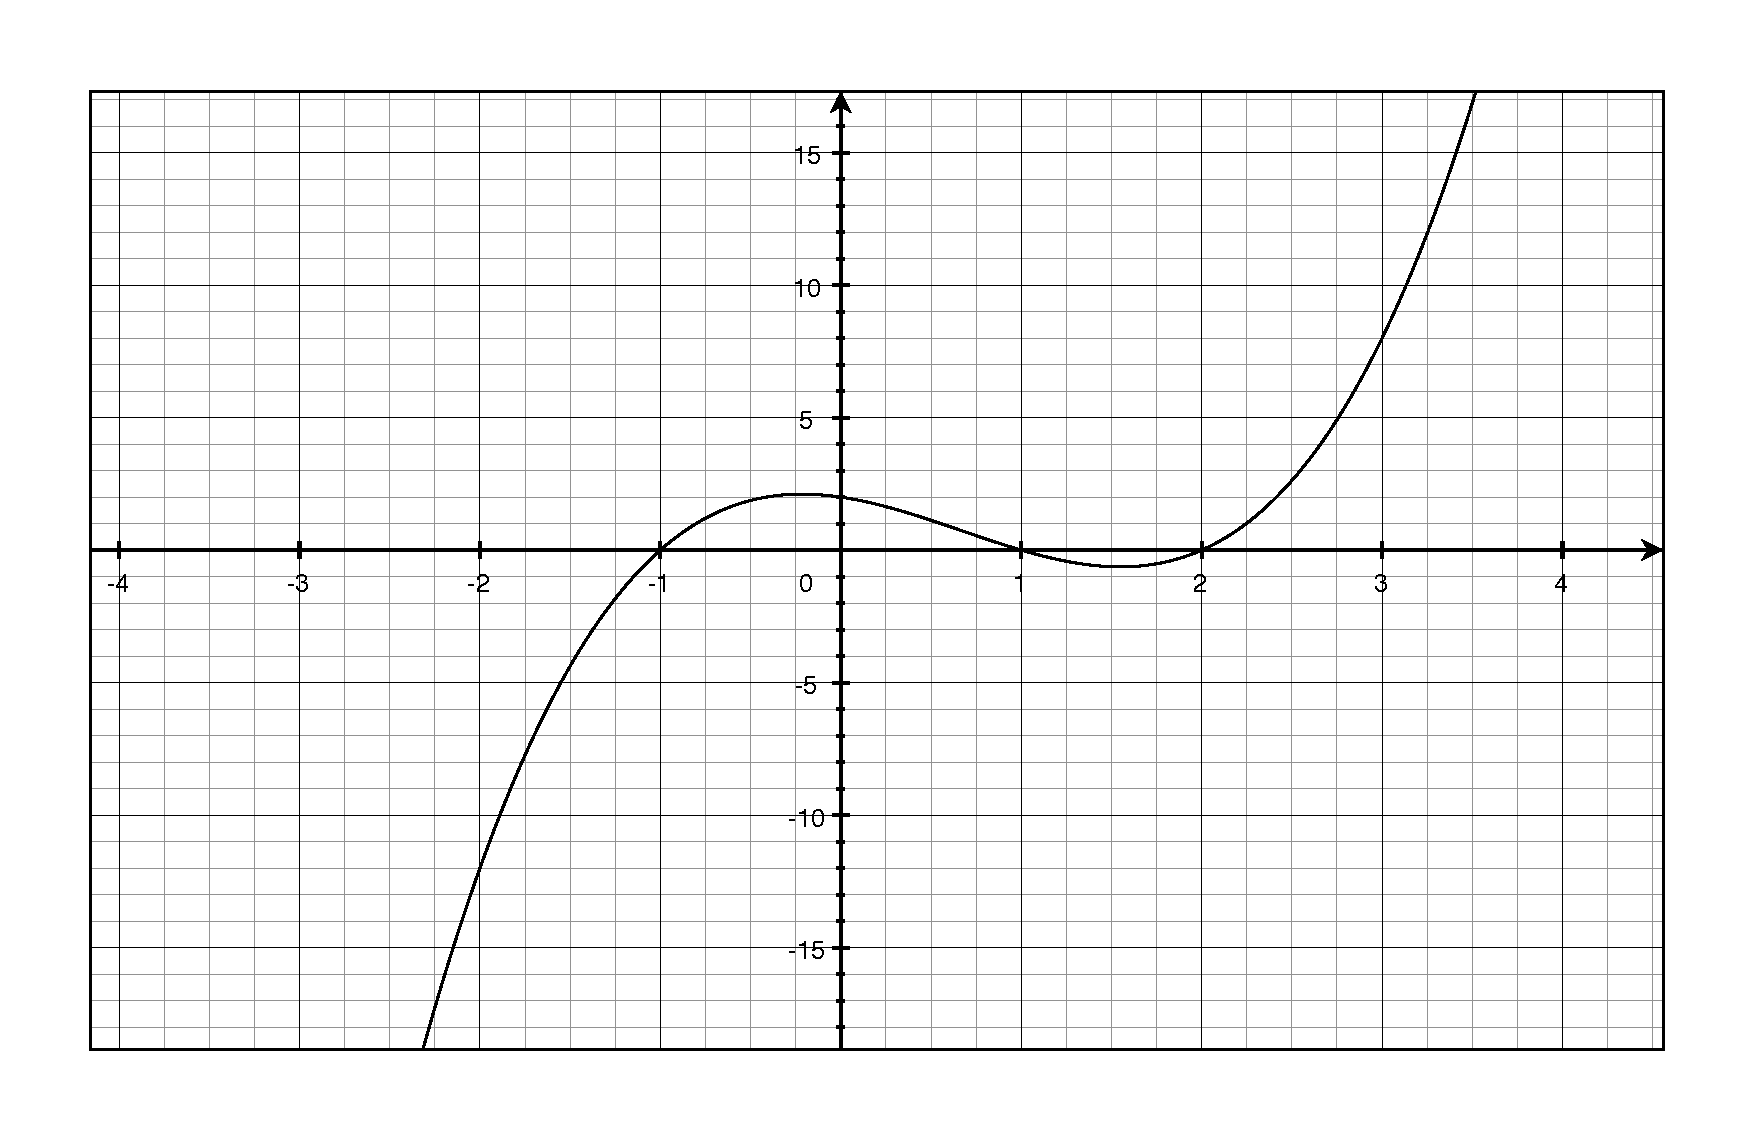
\includegraphics[width=7cm,height=5cm]{question_13.eps}
  \caption*{Question 13}
\end{figure}

\item[14]
\[
  P(x) = -x(x-1)(x-3)^3
\]

The sign is negative because $P(x)$ goes to $-\infty$ as $x$ goes to $\infty$.  Just as in the previous problem, you
could multiply the polynomial by a constant or add additional factors and get a different polynomial that also works.

A few points:
\begin{tabular}{|c|c|c|c|c|}
\hline
  x & -1  & 0 & 2 & 4 \\
\hline
  y & 128 & 0 & 2 & -12 \\
\hline
\end{tabular}

\begin{figure}[H]
  \centering
  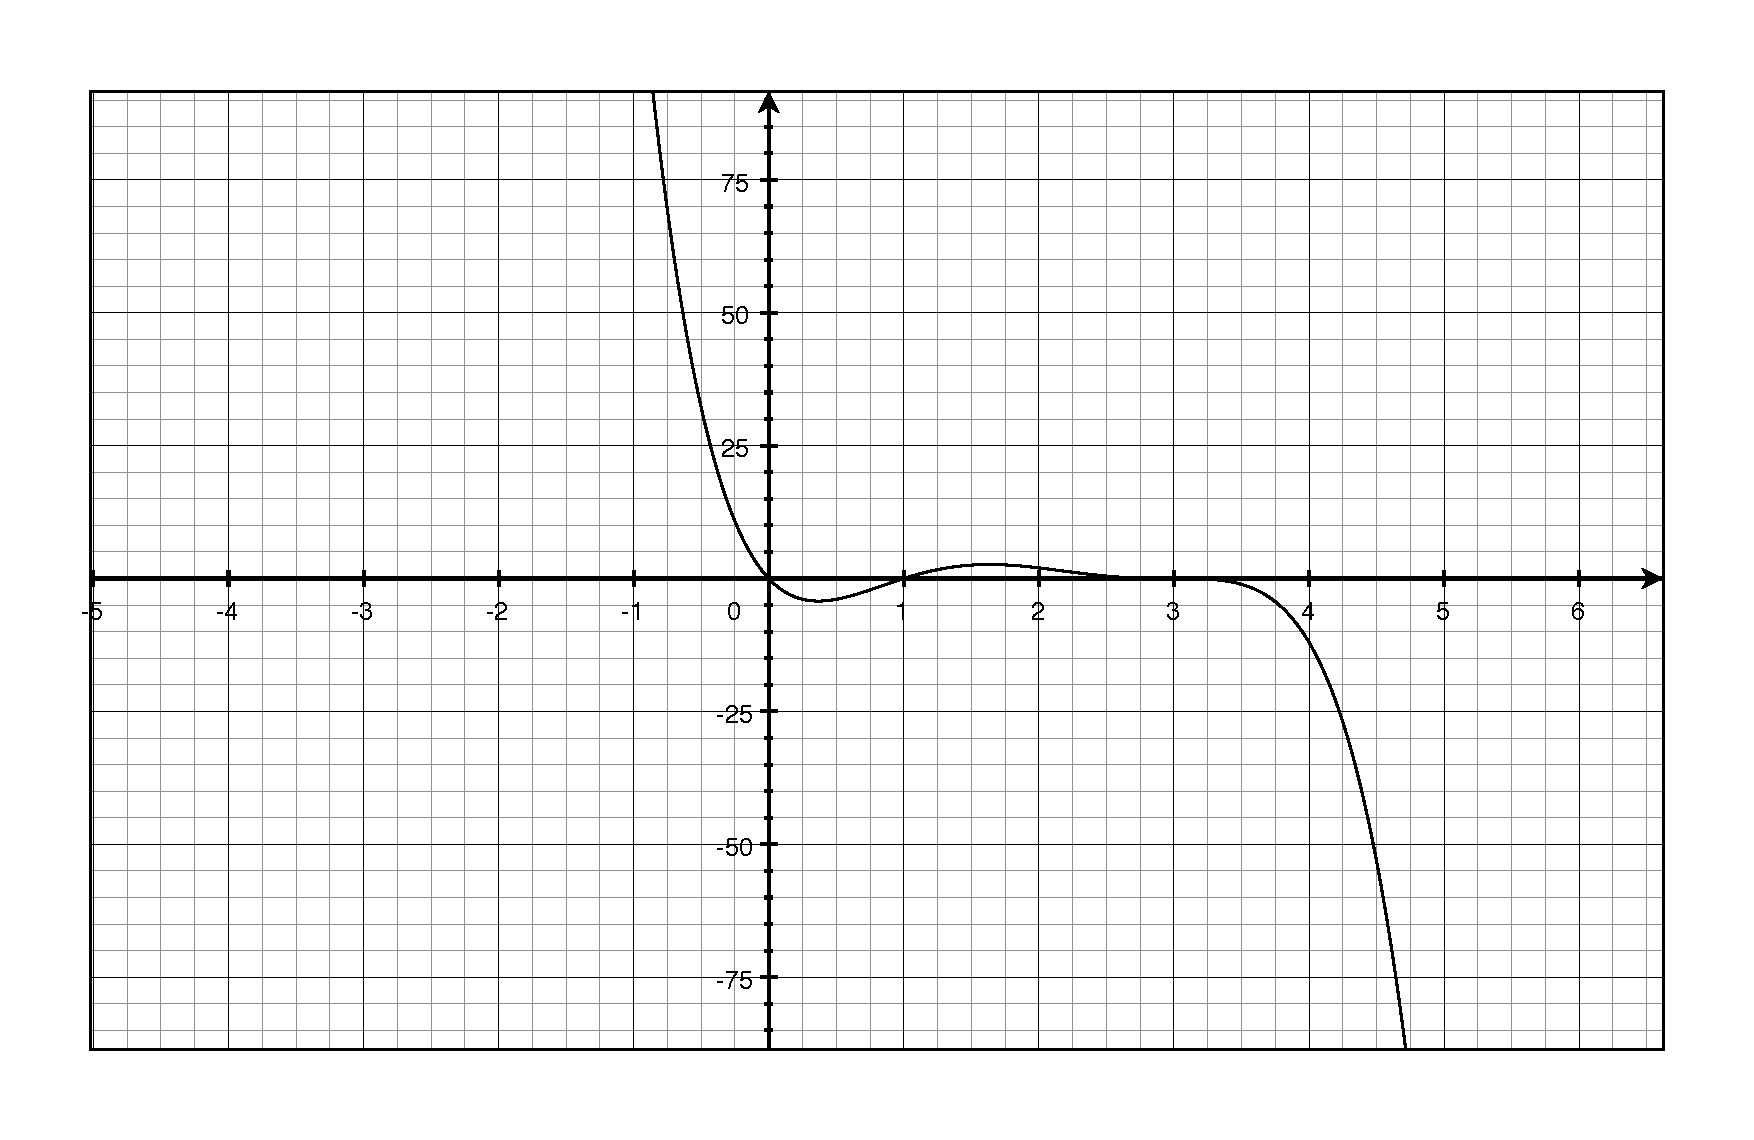
\includegraphics[width=7cm,height=5cm]{question_14.eps}
  \caption*{Question 14}
\end{figure}

\item[15]
The polynomial will look like this: 
\[
  P(x) = a(x-1)(x-2)(x+2) \\
\]

We need to use $P(0) = 2$ to figure out what $a$ is:
\begin{align*}
  a(0-1)(0-2)(0+2) &= 2 \\
  4a &= 2 \\
  a &= \frac{1}{2} \\
\end{align*}

So the function is: $P(x) = \dfrac{1}{2} (x-1) (x-2) (x+2)$

A few points:
\begin{tabular}{|c|c|c|c|c|c|}
\hline
  x & -3  & -1 & 0 & 3/2  & 3 \\
\hline
  y & -10 & 3  & 2 & 7/16 & 5 \\
\hline
\end{tabular}

\begin{figure}[H]
  \centering
  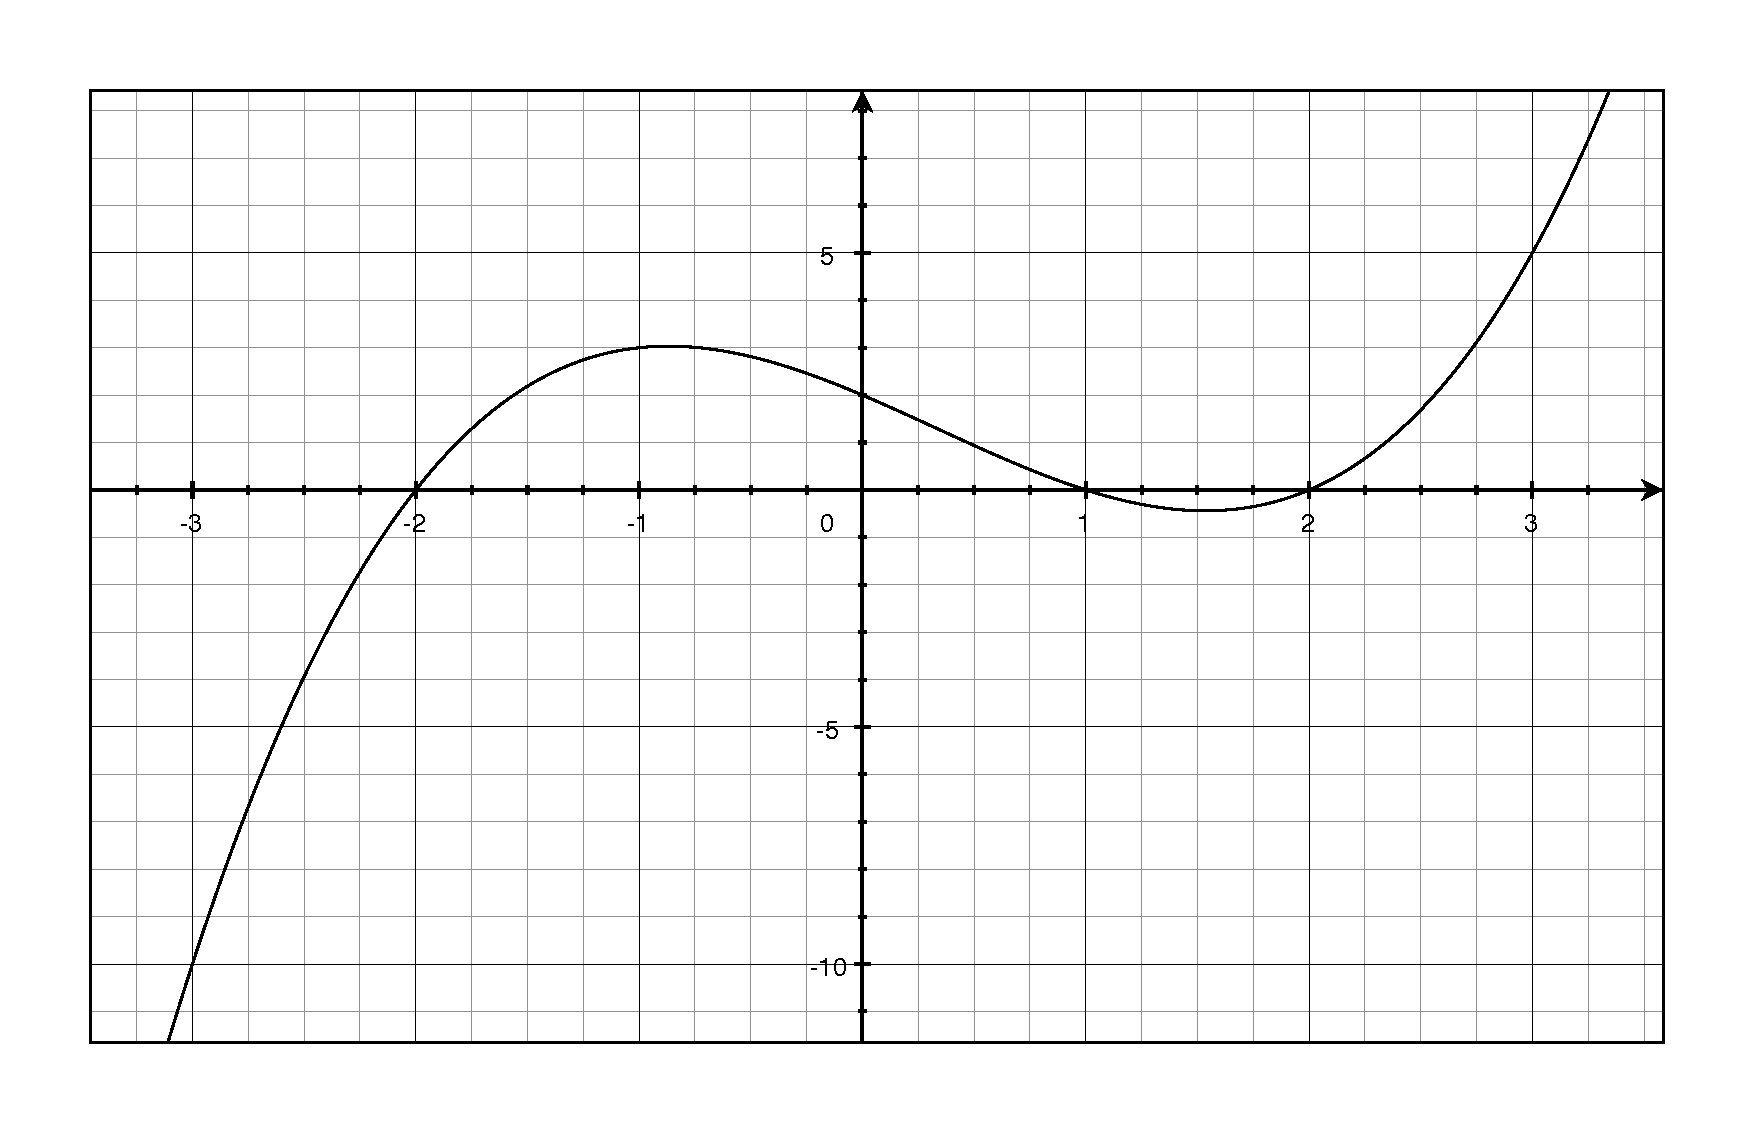
\includegraphics[width=7cm,height=5cm]{question_15.eps}
  \caption*{Question 15}
\end{figure}

\end{description}

\fi

\section{Extra Credit}

\begin{questions}

\question


Suppose you were asked to solve the following two problems on a test:
\begin{itemize}
  \item Find the remainder when $6x^{1000} - 17x^{562} + 12x + 26$ is divided by $x+1$
  \item Is $x-1$ a factor of $x^{567} - 3x^{400} + x^9 + 2$?
\end{itemize}

Obviously, it's impossible to solve these problems by dividing because the polynomials are of such large degree.  Use
the {\em Remainder Theorem} and/or the {\em Factor Theorem} to solve these problems without actually dividing.

({\em from Stewart/Watson/Redlin})

\begin{solution}
Usually the remainder and factor theorems are helpful because they let you use synthetic division to avoid the hard work of
evaluating the polynomial.  In this problem, however, it's the other way around.  Evaulating the polynomials at $1$ and
$-1$ is easy, and doing so will give you the remainder which lets you answer the questions.

\begin{itemize}
  \item For the first equation, $f(-1) = 6 - 17 - 12 + 26 = 3$, so the remainder is $3$.
  \item For the second equation, $f(1) = 1 - 3 + 1 + 2 = 1$, so $x-1$ is not a factor of $f(x)$.
\end{itemize}

\end{solution}

\end{questions}

\ifprintanswers
\else
\vspace{4 cm}

{\em While there is a lower class, I am in it, while there is a criminal element, I am of it, and while there is a soul in prison, I am not free.}

\vspace{.1 cm}
\hspace{1 cm} --Eugene V. Debs

\fi

\end{document}

